\section{The Privacy Dilemma in Single Sign-On}
\label{sec:challenge}

In this section, we describe the challenges for developing privacy-preserving SSO systems and provide an overview of the solutions proposed in UPRESSO.



\subsection{Basic Security Requirements of SSO}
\label{subsec:basicrequirements}
Both the designs of SSO protocols and the implementations of SSO systems are challenging ~\cite{SPRESSO},
%SSO allows users to leverage their existing accounts in the IdP to access services at the RPs.
%However, building such a system is considered challenging~\cite{SPRESSO}, as several design and implementation 
and various vulnerabilities have been found in existing systems~\cite{SomorovskyMSKJ12,WangCW12,ArmandoCCCPS13,ZhouE14,WangZLLYLG15,WangZLG16,YangLLZH16,MainkaMS16,MohsenS16,MainkaMSW17,YangLCZ18,YangLS17,ShiWL19}.
With these vulnerabilities, the adversaries break the security of SSO systems and achieve the following two goals~\cite{SPRESSO}:
%In SSO systems, the adversaries' goals described in~\cite{SPRESSO} to break the secure authentication are:
\begin{itemize}
\item \textbf{Impersonation}: Adversary logs in to an honest RP as the victim user. %The adversary might achieve the goal by obtaining a user's identity proof in the ways, such as stealing the proof (from the unprotected HTTP transmission), forging the valid proof (if the integrity is not guaranteed), leading the user to upload a proof valid for other RPs (the proof is not bound with specific RP).
\item  \textbf{Identity injection}: A victim user logs in to an honest RP under the adversaries' identity. %The adversary might achieve this goal by replacing the identity transmitted from IdP to RP or lead the user uploads the malicious identity proof in various ways (e.g., CSRF).
\end{itemize}

We summarize basic requirements of SSO systems based on existing theoretical analysis~\cite{ArmandoCCCT08,FettKS16, FettKS17} and practical attacks~\cite{SomorovskyMSKJ12,WangCW12,ArmandoCCCPS13,ZhouE14,WangZLLYLG15,WangZLG16,YangLLZH16,MainkaMS16,MohsenS16,MainkaMSW17,YangLCZ18,YangLS17,ShiWL19} on SSO systems. These basic requirements focus on  functions and security of SSO systems, and are as follows: %not considering privacy protection. They are as follows:
%Based on the formal analysis~\cite{ArmandoCCCT08,FettKS16, FettKS17} of SSO protocls (e.g.,SAML, OAuth and OIDC) and the study of existing attacks, we summarize basic requirements that we believe a secure SSO platform which means, 1)RP is always able to identify the user; 2)the system should be protected from forementioned attacks, should meet.

\vspace{1mm}\noindent\textbf{User identification.} When a user logs in to a same RP multiple times, the RP should be able to associate these logins to provide a continuous and personalized service to that user. %The anonymous SSO schemes~\cite{ElmuftiWRR08,WangWS13,HanCSTW18} are also proposed to achieve that the user's identity is unknown the neither the IdP nor the RP. However, these schemes are not focally concerned in this paper as the completely anonymous SSO systems are not suitable to the currently web application where the RP need to know the user's identity to provide the personally service. The anonymous SSO schemes are discussed in Section~\ref{sec:related}.

\vspace{1mm}\noindent\textbf{Receiver designation.} The receiver designation requires that the identity proof should  be  transmitted only to the RP (and user) that the user visits, and be bound to this RP so that it will accepted only by this RP. %(through the user). Otherwise, the adversaries who is able to achieve honest user's identity proof for honest RP, have the ability to conduct impersonation attack~\cite{ChenPCTKT14, WangZLG16}


\begin{comment}
\vspace{1mm}\noindent\textbf{Identification.} %Identification is the main feature of SSO system, which enables the RP to identify the user.
After a successful SSO authentication, the RP should be able to uniquely identify the user. When a user logs in to a same RP multiple times, the RP should be able to associate these logins to provide a continuous and personalized service to that user. This is an essential requirement for any authentication mechanism. In SSO, this indicates that a same unique user identifier should be derived from multiple identity proofs of the user by the RP. In OIDC, for example, a user obtains different PPIDs from the IdP, each for a different RP.


\vspace{1mm}\noindent\textbf{Binding.} Each identity proof should be bound to one RP so that it will be accepted only by that RP. Otherwise, the identity proof may be abused to impersonate the victim user at other honest RPs~\cite{ChenPCTKT14, WangZLG16}. To achieve such binding in OIDC, the IdP embeds the identifier of the target RP in the identity proof and signs it with its private key. When receiving an identity proof, the RP needs to check if it is the intended receiver.

\vspace{1mm}\noindent\textbf{Confidentiality.} The identity proof should be securely returned to the requesting RP (and the user). Otherwise, an adversary who obtains an identity proof can impersonate the user at the RP specified in the identity proof~\cite{ChenPCTKT14,FettKS16,WangZLG16}. Currently, OIDC adopts TLS to ensure the confidentiality during the transmission. However, additional checking should be performed during the generation of the identity proof by the IdP and the transmission of the identity proof by the user and its trusted user agent.
\end{comment}

\vspace{1mm}\noindent\textbf{Integrity.} Only the IdP is able to generate a valid identity proof,
     no other entity should be able to modify or forge it~\cite{WangZLG16} without being found. And, the honest RP should only accept the valid identity proof.
    %Otherwise, an adversary could modify user identifier in the proof to launch impersonation or identity injection attacks. In OIDC, for example, the IdP signs identity proofs with its private key to provide integrity~\cite{WangCW12, SomorovskyMSKJ12}.

These basic requirements are the minimum properties that an SSO system has to provide.
User identification is necessary for all services except the anonymous systems which will be discussed in Section~\ref{sec:related},
 therefore RPs should be able to identify the user with the help from IdP.
While either the receiver designation and integrity not satisfied, the impersonation and identity injection will exist in the SSO systems.
For example, without the receiver designation,  the adversaries cloud use the leaked identity proof to impersonate the victim user at an honest RP~\cite{ChenPCTKT14,FettKS16,WangZLG16}, and  make the victim RP  incorrectly accept the identity proof intended for other RP, which allows the adversary to perform impersonation directly or inject the identity proof in the web session between the victim user and honest RP with other web attacks (e.g., CSRF);
while without integrity, the impersonation and identity injection attacks will be more easier as an adversary could directly modify user's identifier in the identity proof. % to launch impersonation or identity injection attacks
 
\begin{comment}
\vspace{1mm}Breaking the above requirements will lead to some attacks.
in SSO systems, the adversaries' goals described in~\cite{SPRESSO} to break the secure authentication are:
(1) \textbf{Impersonation}: Adversary logs in to the honest RP as an honest user. The adversary might achieve the goal by obtaining a user's identity proof in the ways, such as stealing the proof (from the unprotected HTTP transmission), forging the valid proof (if the integrity is not guaranteed), leading the user to upload a proof valid for other RPs (the proof is not bound with specific RP).
(2) \textbf{Identity injection}: Honest user logs in to the honest RP under adversaries' identity. The adversary might achieve this goal by replacing the identity transmitted from IdP to RP or lead the user uploads the malicious identity proof in various ways (e.g., CSRF).

Or break identification will lead to \textbf{anonymity}. the anonymous SSO schemes~\cite{ElmuftiWRR08,WangWS13,HanCSTW18} are also proposed to achieve that the user's identity is unknown the neither the IdP nor the RP. However, these schemes are not focally concerned in this paper as the completely anonymous SSO systems are not suitable to the currently web application where the RP need to know the user's identity to provide the personally service. The anonymous SSO schemes are discussed in Section~\ref{sec:related}.
\end{comment}

\subsection{The Privacy Dilemma and Existing Attempts}
\label{subsec:challenges}
\begin{comment}
In UPRESSO, the adversaries' goals to break the secure authentication are as follows:
\begin{itemize}
\item Impersonation attack: Adversary logs in to the honest RP as an honest user. The adversary might achieve the goal by obtaining a user's identity proof in the ways, such as stealing the proof (from the unprotected HTTP transmission), forging the valid proof (if the integrity is not guaranteed), leading the user to upload a proof valid for other RPs (the proof is not bound with specific RP).
\item Identity Injection: Honest user logs in to the honest RP under adversaries' identity. The adversary might achieve this goal by replacing the identity transmitted from IdP to RP or lead the user uploads the malicious identity proof in various ways (e.g., CSRF).
\end{itemize}
\end{comment}



%A privacy-preserving SSO needs to prevent both IdP-based access tracing and RP-based identity linkage.
In addition to the basic requirements, a privacy-preserving SSO system should prevent the IdP-based access tracing %login tracing 和 access tracing 没有已经广泛使用的说法
and RP-based identity linkage. 
In details, the privacy-preserving SSO system should prevent the curious IdP from obtaining any information that could identify the user's accessed RP (e.g., RP's identifier and URL),
and prevent  the collusive RPs from correlating the user's identifiers at different RPs. % in the identity proof.
%the user's identifiers provided by IdP for one user should never be same or derivable to each other.

The privacy-preserving requirements need to be integrated into the basic requirements, to protect the user privacy under the prerequisite that the correct functions and security of SSO systems are ensured.
The privacy-preserving user identification requires IdP to provide a user's identifier ($PID_U$) to help the RP in identifying the user locally,
 under the prerequisites that the curious IdP can never identify the visiting RP and the collusive RPs cannot find the correlation between $PID_U$s for a user.
The privacy-preserving receiver designation requires IdP (or the user) to bind an identity proof with an RP and send it only to this RP,
 while IdP can never identify which RP is visited by the user. 
  
%To conform the requirements of user identification and receiver designation, which is to be validated by the RP, the identity proof must contains (or is related with) specific RP identifier (e.g. $ID_{RP}$) and user identifier (e.g. $ID_U$). However, as the identity proof is generated by the IdP, the $ID_{RP}$ and $ID_U$ allows the IdP to know which RP the user accessed. Moreover, as the identity proof is verified by the RP, the colluded RPs are able to link the same user. Therefore, the key point of privacy-preserving SSO system is to hide the $ID_{RP}$ and $ID_U$ while generating the identity proof.



We define that the simplified identity proof model as the tuple $<ID_{RP}, ID_U>$. For each entity in the system, everyone knows the full tuple is able to trace the user (by IdP-based access tracing and RP-based identity linkage). It should be concerned that the RP always know the $ID_{RP}$. We can transform the problem into hiding the full tuple to IdP and RP.

In traditional SSO systems, the tuple is always exposed to both IdP and RP, so that they do not protect user from any kind of tracing. In OIDC, $PPID$ is adopted to hide the $ID_U$ from RP by using the RP-unique identifier. In SPRESSO, the identity proof is generated for a encrypted $ID_{RP}$ so that the IdP is unable to obtain the full tuple which avoids the IdP-based access tracing. In BrowserID, the generation of identity proof is split and the responsibility of binding it to RP is shifted to user, which also avoids the IdP-based access tracing. However OIDC allows the full tuple is exposed to IdP, while SPRESSO and BrowserID allows the RP obtains the full tuple, all of which cause the user to be tracked.

The key challenge is that there is no simple way to hide the full tuple to both IdP and RP. To tackle this problem, it requires the IdP to generate pairwise identifiers for a user and bind them to pseudo RP identifiers that seem random to IdP, in a way that user identifiers are unique at one RP but different at different RPs and user identifiers bound to pseudo identifiers of the same RP can be associated by that RP.


\begin{figure}
  \centering
  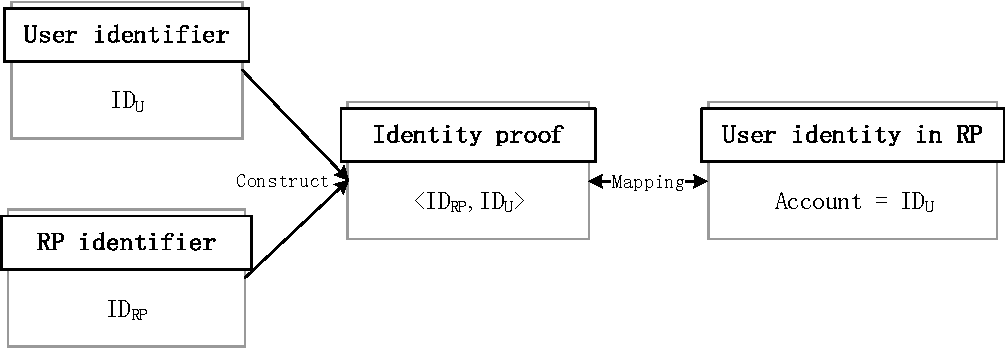
\includegraphics[width=\linewidth]{fig/mapping1.pdf}
  \caption{Traditional SSO.}
  \label{fig:TraditionalSSO}
\end{figure}
\begin{figure}
  \centering
  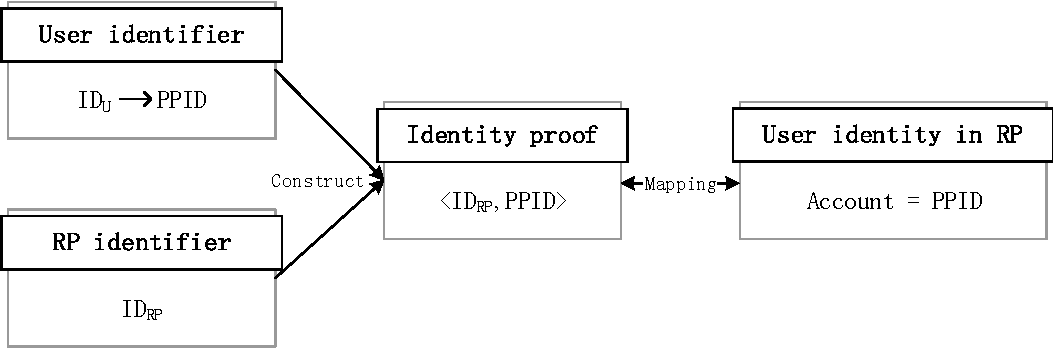
\includegraphics[width=\linewidth]{fig/mapping2.pdf}
  \caption{PPID.}
  \label{fig:PPID}
\end{figure}
\begin{figure}
  \centering
  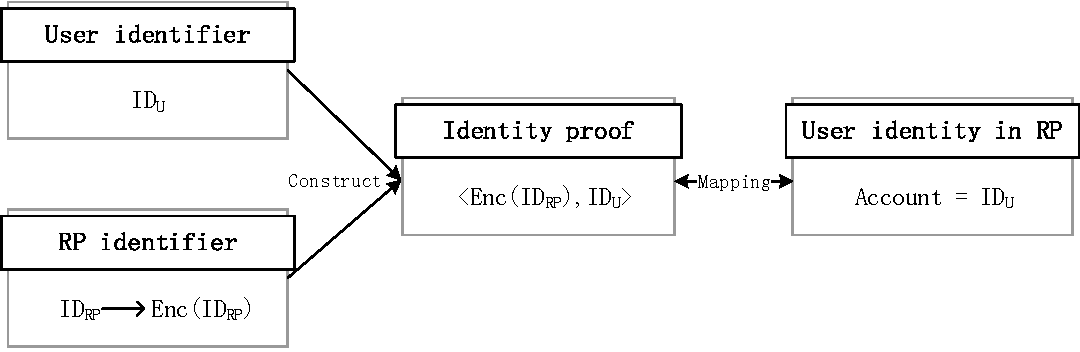
\includegraphics[width=\linewidth]{fig/mapping3.pdf}
  \caption{SPRESSO.}
  \label{fig:SPRESSO}
\end{figure}
\begin{figure}
  \centering
  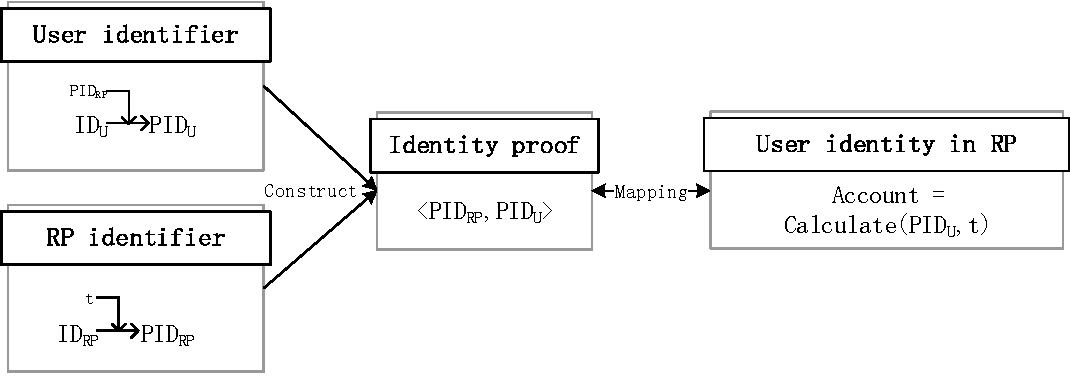
\includegraphics[width=\linewidth]{fig/mapping5.pdf}
  \caption{Our scheme.}
  \label{fig:Ourscheme}
\end{figure}
\begin{comment}

{\color{red}
The root reason that existing SSO systems suffer from privacy attacks is that they cannot meet secure authentication and privacy protection requirements
%why the current schemes for privacy-preserving SSO systems cannot deal with the IdP-based access tracing and RP-based identity linkage
at the same time. %is that no existing SSO systems satisfy all the requirements of secure authentication and privacy.
For secure authentication, the identity proof should be bound to a specific RP identifier and a specific user identifier. %The secure authentication requirements must be satisfied by all the SSO systems to avoid the potential attacks.
However, for privacy protection, the privacy-preserving SSO systems require (i) the RP identifier to be one-time and indistinguishable to IdP, and (ii) the user identifier to be globally indistinguishable to IdP but identifiable to the RP. %The ignoring of any privacy requirements is to eventually result in the user being tracked.

Several privacy-preserving schemes have been proposed to meet the privacy requirements while supporting secure authentication, however, they cannot satisfy both privacy requirements at the same time. For example, OIDC adopts PPID as an RP-specific user identifier, but for secure authentication, it has to use a unique RPID to generate the identity proof and thus suffers from IdP-based tracing. On the contrary, SPRESSO encrypts the RP domain to generate a one-time RPID that hides the RP identity against IdP, but it uses static user identifier in identity proof and thus is vulnerable to RP-based linkage. BrowserID takes a different approach by binding the globally unique user identifier with an asymmetric key pair and letting the user to sign RP's domain with the private key. However, the unique signature can be used to link the RPs accessed by the same user in RP-based linkage.
%However, is there a simple way to satisfy the privacy requirements by combining the exiting schemes together, for example using one-time encrypted RPID in OIDC or using PPID in SPRESSO?

The key challenge is that there is no simple way to bind the identity proof to a user's identity without exposing the requesting RP's identity to IdP. To tackle this problem, it requires the IdP to generate pairwise identifiers for a user and bind them to pseudo RP identifiers that seem random to IdP, in a way that user identifiers are unique at one RP but different at different RPs and user identifiers bound to pseudo identifiers of the same RP can be associated by that RP.
%without knowing the RP identifier. Such pairwise user identifiers should be uniquely bound to an .
%so that the pairwise user identifier changes and underivable even in the same RP.
}
\end{comment}

\begin{comment}
However, these two requirements for privacy preservation,  conflict with the basic requirements on SSO as follows: %, resulting in the following problems in SSO systems:
\begin{itemize}
	\item \textbf{No Identification.} In the privacy-preserving SSO, IdP doesn't know the RP's identifier, therefore fails to provide the  pairwise user's identifier which is unchanged in one RP but different in different RPs (e.g. PPID in OIDC and SAML~\cite{OpenIDConnect,SAMLIdentifier}). Also, the user's unique identifier (e.g., the email address in BrowserID~\cite{BrowserID} and SPRESSO~\cite{SPRESSO}) should not be sent to the RP, otherwise the collusive RPs may perform the identity linkage with the same identifier.
%User account is the unique identifier for the RP to provide the individual services for each user.
%In SSO systems, RP derives the user account from the identifier (i.e., PPID in OIDC) provided by the identity proof.
%However, in privacy-preserving SSO systems, IdP must provides the pairwise user identifier (never same for different RPs) without knowing the identity of RP.
%Therefore, IdP is only able to provide different user identifier for user's multiple logins at the same RP, which makes RP fail to provide the consecutive and individual services.

%Each RP provides the individual services for each user based on the unique account. In SSO systems, RP derives the user account from the identifier (i.e., PPID in OIDC) in the identity proof. With the correct RP identifier, IdP ensures the PPID is unique for the user's multiple logins at the same RP. However, when IdP fails to obtain the exact RP identifier, IdP is only able to provide different PPIDs for user's multiple logins at the same RP, which makes RP fail to provide the consecutive and individual services.
	\item \textbf{No Binding.} IdP, who doesn't know the RP's identifier, fails to bind the identity proof with a specified RP.
On receiving the identity proof not bound to it, the RP either (1) rejects the proof and halts its service; or (2) accepts the proof.
The second case will make  one identity proof  be accepted by multiple RPs, which results in the misuse of identity proof for impersonation attacks and identity injection~\cite{ChenPCTKT14,FettKS16,WangZLG16}.
    \item \textbf{No Confidentiality.}
    The potential leakage of the identity proof exists, as:
    (1) No reliable checks (from the IdP and user) during the generation of identity proof, as the IdP lacks the correct RP identifier to retrieve the exact information from the local storage,
     while the user fails to obtain the correct RP name (or URL) from IdP for the check.
     Therefore, the malicious RP may cheat user about its identity to request the identity proof for another RP without being found by the IdP and user.
     (2) Lack of correct URL for the transmission, as without the correct RP identifier, IdP fails to extract the correct (locally stored) URL.
      The trusted user agent may transmit the identity proof to the incorrect URL hold by the adversary.
    The leakage of identity proof may result in the impersonation attacks~\cite{ChenPCTKT14,FettKS16,WangZLG16}.
\end{itemize}
Due to these conflicts, no existing SSO systems satisfy the two privacy requirements.
IdP-based access tracing exists in the implementations based on SAML, OAuth, and OIDC, as IdP knows identifiers accessed by the user.
RP-based identity linkage is not prevented in BrowserID~\cite{BrowserID} and SPRESSO~\cite{SPRESSO}, as the email address is sent to all the RPs.
\end{comment}





\subsection{The Principles of UPRESSO}
\label{subsec:solutions}
In this work, we present UPRESSO to defend against both IdP-based access tracing and RP-based identity linkage privacy attacks with enhanced security for identification, binding and confidentiality. %to satisfy the basic requirements of SSO systems.
Since the integrity requirement for identity proof is orthogonal to the privacy requirement, UPRESSO adopts the same signature-based integrity mechanism of OIDC.
Next, we overview the new privacy-preserving user identification and receiver designation schemes in UPRESSO.


\vspace{1mm}\noindent \textbf{Trapdoor user identification.} The trapdoor identification make the RP possible to transform the user's identity proof into the constant Account in RP, even the $ID_U^{Proof}$ (user identifier in identity proof) is changing with the $PID_{RP}$, which is to prevent the RP-based identity linkage.

\vspace{1mm}\noindent \textbf{Transformed receiver designation.} The pseudonymous receiver uniqueness allows the IdP to generate the identity proof bound to specific RP without knowing any straightforward RP information but a transformed RP identifier, and the identity proof is bound to the transformed identifier. As the IdP does not the RP’s identity, responsibility of url checking should be shifted from IdP to RP, which guarantees the identity proof is only sent to the bound RP.

\begin{comment}
\vspace{1mm}\noindent \textbf{Trapdoor identification.}
The trapdoor identification make the RP possible to transform the user's identity proof into the constant $Account$ in RP, even the $ID_U^{Proof}$ (user identifier in identity proof) is changing with the $PID_RP$, which is to prevent the RP-based identity linkage.
The entity with the trapdoor can derive the unique user account associated with an RP from different identifiers in multiple identity proofs generated when the user logs in to that RP multiple times.
%The trapdoor-existing identification requires that the user identifier generated by IdP should be never same in each authentication as the RP's identity is unknown to IdP and the identifier should be derivable to the specific account unchanged in RP with the trapdoor.
%In UPRESSO, the user's account at an RP is a function of the RP's original identifier and the user's unique identifier.
%The generation of this unique user account consists of two steps executed by the IdP and RP independently to prevent not only the IdP from obtaining the RP identifier but also the RP from inferring the unique user identifier.
%In the first step, IdP generates a PPID with the user identifier and the RP identifier transformation. Since the RP identifier transformations are independent in multiple login flows, the PPIDs generated by the IdP in these flows are different.
%which results in different PPIDs for multiple logins at a RP as various transformations are adopted.
%In the second step, the requesting RP adopts the trapdoor of the transformation of the RP identifier to derive the unique user account from the PPIDs. Moreover, the accounts of a user at various RPs are different, as the original RP identifiers are different, which prevents the identity linkage.

\vspace{1mm}\noindent \textbf{Transformed binding.}
The transformed binding allows the IdP to generate the identity proof bound to specific RP without knowing any straightforward RP information.
The identity proof is bound to the transformation of a RP identifier, which allows the RP to check whether the identity proof is for it while preventing the IdP from inferring the original RP identifier. Only the identity proof bound to a fresh transformation of its identifier will be accepted by the RP.
%The transformed binding requires that the RP should provide the one-time transformed identifier, unlinkable to the RP's unique identifier without trapdoor and the identity proof should be bound with the one-time identifier.
%In UPRESSO, the transformation of the RP identifier is generated by the user and RP cooperatively, which prevents the adversary from constructing a same or related transformation for different RPs. The IdP obtains the transformation of an RP identifier and binds it to the identity proof.
%the identity proof is bound with a transformation of the RP's identifier by the IdP, who cannot infer the original identifier from the transformation.

%Moreover,
%Otherwise, the identity proof will be accepted by multiple RPs, which results in the misuse of the proof for the impersonate attack.

\vspace{1mm}\noindent \textbf{User-centric confidentiality.}
User-centric confidentiality shifts the responsibility of url checking from IdP to user agent, which guarantees the identity proof is only sent to the bound RP. The user-centric confidentiality should relies on the trustful user agent and IdP issued RP identity certificate.
%In UPRESSO, the user sends the authentication request to the IdP to generate an identity proof for the requested RP identifier transformation. To ensure the identity proof is securely returned to the requesting RP, UPRESSO adopts a user-centric confidentiality check, which requires the user to extract RP's identifying information (e.g., URL, name and RP identifier) from the RP certificate issued by a trusted entity (e.g., IdP). Therefore, it is impossible for an adversary to request the identity proof on behalf of others or intercept others' identify proofs with a forged return URL.
\end{comment}

To combine these three principles into one system, we propose novel identifier generation schemes to dynamically generate transformed RP identifier and trapdoor identity proof, which makes the RP's information never exposed to the IdP during the authentication and RP able to derive the unique user $Account$ from identity proof. Moreover, both the RP identifier transforming and identity proof transformation (including url check) require the trustful user agent. We do not explain how to finish each principle here, it will be explained in Section \ref{subsec:overview}.
%\vspace{1mm} \textbf{xxx xxxxx xxxxxxx
%(1) How to combine these three principles into one system?
%(2) Why these principles protect privacy while ensure security?
%(3) we do not explain how to finish each principle here, it will be explained in Section \ref{subsec:overview}.}









